\documentclass[final,x11names]{beamer}

\usecolortheme{seagull}
% headline colors and fonts
\setbeamercolor{headline}{fg=white,bg=DodgerBlue4}
\setbeamercolor{title in headline}{fg=white}
\setbeamercolor{author in headline}{fg=lightgray}
\setbeamercolor{institute in headline}{fg=lightgray}
\setbeamercolor{logo in headline}{fg=black,bg=lightgray}
\setbeamercolor{separation line}{bg=black}

% footline colors and fonts
\setbeamercolor{footline}{fg=gray!20,bg=DodgerBlue4}
\setbeamerfont{footline}{size=\small}

% body colors and fonts
\setbeamercolor*{normal text}{fg=black,bg=white}

% block environment
\setbeamercolor*{block body}{bg=gray!3,fg=black}
\setbeamercolor*{block title}{fg=white,bg=DodgerBlue4}
\setbeamerfont{block title}{size=\large,series=\bf}

% example environment
\setbeamercolor*{example title}{fg=white,bg=blue}
\usefonttheme{serif}
\setbeamerfont{example title}{size=\large,series=\bf,bg=DodgerBlue4,fg=white}


\setbeamercolor{alerted text}{fg=orange}

%\setbeamertemplate{itemize items}[triangle]
\setbeamertemplate{navigation symbols}{}  % no navigation on a poster

%%%%%%%%%%%%%%%%%%%%%%%%%%%%%%%%%%%%%%
%
% Block Style
%
%%%%%%%%%%%%%%%%%%%%%%%%%%%%%%%%%%%%%%
\setbeamertemplate{block begin}{
  \vskip.75ex
  \begin{beamercolorbox}[leftskip=1cm,colsep*=.75ex,rounded=true,shadow=true]{block title}%
    \usebeamerfont*{block title}\textsf\insertblocktitle
  \end{beamercolorbox}%
  {\ifbeamercolorempty[bg]{block body}{}{\nointerlineskip\vskip-0.5pt}}%
  \usebeamerfont{block body}%
  \begin{beamercolorbox}[rounded=true,vmode]{block body}%
  %\begin{beamercolorbox}[]{block body}
    \ifbeamercolorempty[bg]{block body}{\vskip-.25ex}{\vskip-.75ex}\vbox{}%
  }
  \setbeamertemplate{block end}{
  \end{beamercolorbox}
}

%%%%%%%%%%%%%%%%%%%%%%%%%%%%%%%%%%%%%%
%
% Header 
%
%%%%%%%%%%%%%%%%%%%%%%%%%%%%%%%%%%%%%%
\setbeamertemplate{headline}{  
  \leavevmode

      \begin{beamercolorbox}[sep=0.1cm,wd=.1\paperwidth,center]{logo in headline}
        \vskip2ex
      \end{beamercolorbox}  
      \begin{beamercolorbox}[sep=1cm,wd=\paperwidth]{headline}
        \usebeamercolor{title in headline}{%
\hspace{1cm}\raggedright\color{fg}\textbf{\textsf{\LARGE{\inserttitle}}}\\[1ex]}
        \usebeamercolor{author in headline}{%
\hspace{1cm}\raggedright\color{fg}\textsf{\large{\insertauthor}}\\[3ex]}
        \usebeamercolor{institute in headline}{%
\hspace{1cm}\raggedright\color{fg}\textsf{\large{\insertinstitute}}\\[1ex]}     
      \end{beamercolorbox}%
      \begin{beamercolorbox}[sep=0.1cm,wd=.18\paperwidth,center]{logo in headline}
     %   \includegraphics[height=5cm]{logos/rwth-hks44}
        \vskip2ex
      \end{beamercolorbox}  
  
  \begin{beamercolorbox}[wd=\paperwidth]{lower separation line head}
    \rule{0pt}{2pt}
  \end{beamercolorbox}
}

%%%%%%%%%%%%%%%%%%%%%%%%%%%%%%%%%%%%%%
%
% Footer
%
%%%%%%%%%%%%%%%%%%%%%%%%%%%%%%%%%%%%%%
\setbeamertemplate{footline}{
  \begin{beamercolorbox}[wd=.9\paperwidth]{upper separation line foot}
    \rule{0pt}{2pt}
  \end{beamercolorbox}
  
  \begin{beamercolorbox}[ht=2.4ex,leftskip=1cm,rightskip=1cm]{footline}%
    Hydrology, Water Resources and Environmental Fluid Mechanics -- 
    Civil, Environmental and Architectural Engineering -- 
    University of Colorado at Boulder --
    Boulder, Colorado 
    \hfill \texttt{cameron.bracken@colorado.edu} 
    \vspace{0.2ex}
  \end{beamercolorbox}

  \begin{beamercolorbox}[wd=\paperwidth]{lower separation line foot}
    \rule{0pt}{2pt}
  \end{beamercolorbox}
}

\usepackage{times}
\usepackage{amsmath,amsthm, amssymb, latexsym}
\boldmath
\listfiles
\usepackage[orientation=landscape,size=a0,scale=1.2,debug]{beamerposter}

\graphicspath{{figures/}}
\title{Interannual Forecasting of Upper Colorado River Flow}
\author{Cameron Bracken$^{1,\,2}$, Balaji Rajagopalan$^{2}$, Edith Zagona$^{1}$}
\institute[CADSWES]{\small$^{1}$Center for Advanced Decision Support for Water and 
    Environmental Systems (CADSWES), $^{2}$Department of Civil Environmental and Water Resources Engineering, University of Colorado at Boulder}
\date{March 31th, 2011}


\begin{document}
  \begin{frame}{} 
    \begin{columns}
      %%%%%%%%%%%%%%%%%%%%%%%%%%%%%%%%%%%%%%%%%%%%%%%%%%%%%%%%%%%%%%%%%%%%
      %
      % Column 1
      %
      %%%%%%%%%%%%%%%%%%%%%%%%%%%%%%%%%%%%%%%%%%%%%%%%%%%%%%%%%%%%%%%%%%%%
      \begin{column}{.33\linewidth}
        
        %%%%%%%%%%%%%
        %%%%% Block 1
        %%%%%%%%%%%%%
        \begin{block}{\large The Upper Colorado River Basin}
			\begin{columns} 
			  \begin{column}{.47\textwidth} 
			    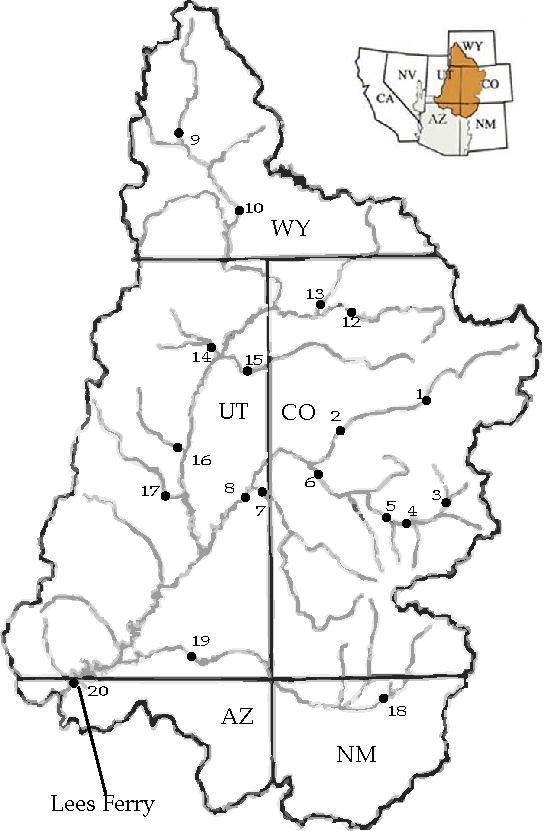
\includegraphics[width=.9\columnwidth]{figs/map1_nodes.pdf}
			    			   \begin{itemize}
			      \item Parts of seven states with an area of 303,450 mi$^2$.  
			      \item Elevations ranging from 200 to 14,200 ft.
			      \end{itemize}
			  \end{column} 
			  \begin{column}{.52\textwidth} 
				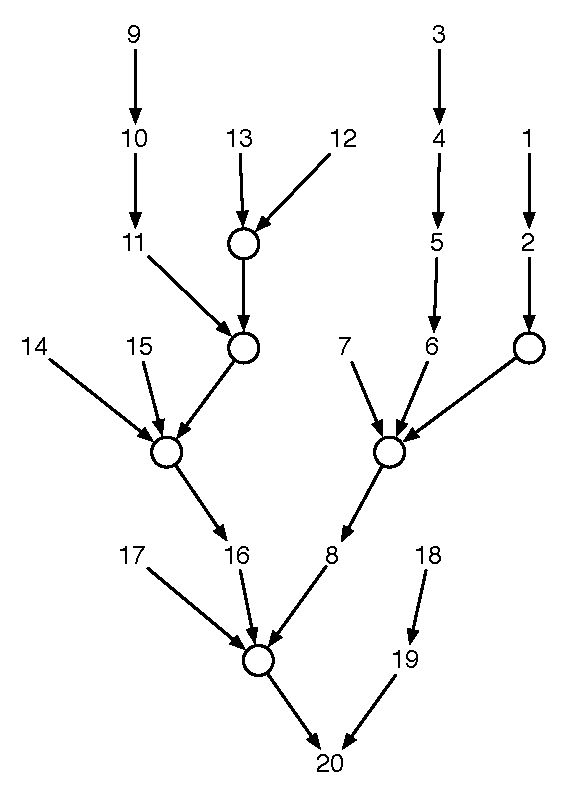
\includegraphics[width=.9\columnwidth]{figs/intervening-to-total-schematic.pdf}
				\begin{itemize}
			      \item Nearly 80\% of the streamflow in the UCRB is due to snowmelt.
			      \item 19 important gages in the Upper Colorado River Basin.
			    \end{itemize}
			  \end{column} 
			  
			\end{columns} 

		\end{block}
		
        %%%%%%%%%%%%%
        %%%%% Block 2
        %%%%%%%%%%%%%
		\begin{block}{\large Current Forecasting Methods}
			\begin{columns} [T]
			  \begin{column}{.5\textwidth} 
			  
			    \begin{itemize}
			    \item Current methods use a blend of snow, soil and climate information 
			          in both physical and statistical models. 
			    \item {\color{orange}The longest lead forecasts currently can only accurately 
			          predict peak season streamflow (Apr-July) about 6 months in advance} 
			          [Regonda et. al. 2006, Bracken et al. 2010].  
			    \end{itemize}
			    
			    \begin{center}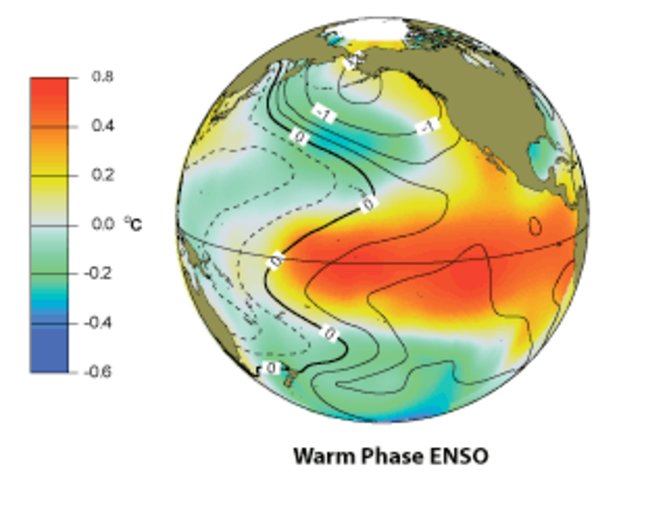
\includegraphics[width=.7\columnwidth]{figs/englobe}\end{center}
			  \end{column} 
			  \begin{column}{.45\textwidth} 
			    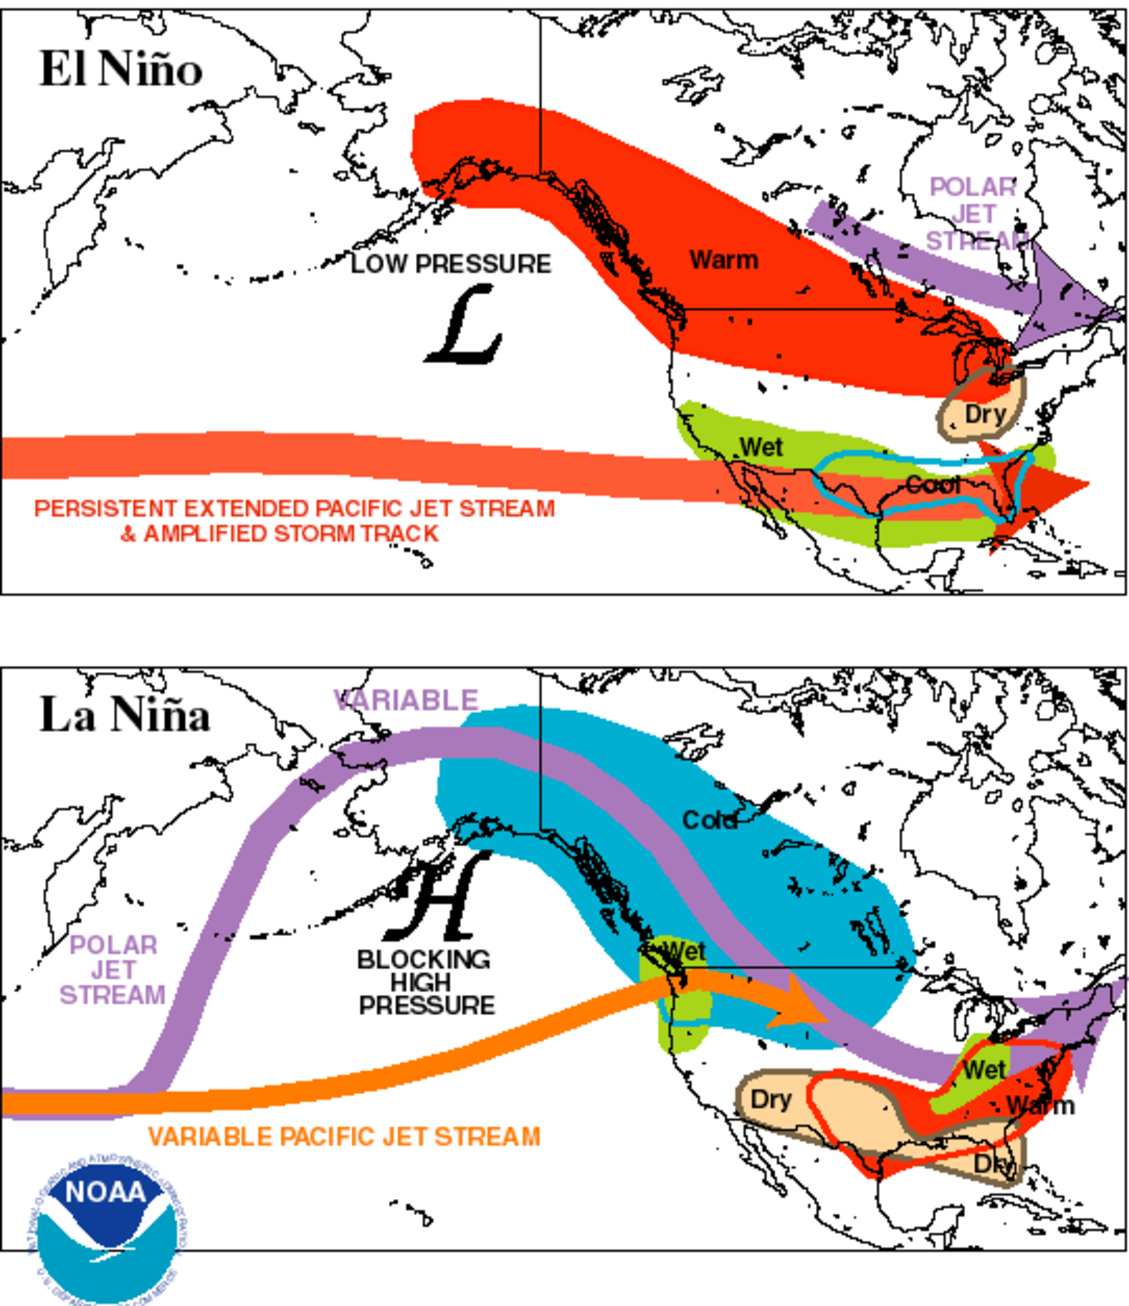
\includegraphics[width=.9\columnwidth]{figs/jetstream} 
			  \end{column} 
			\end{columns}
			\centering
			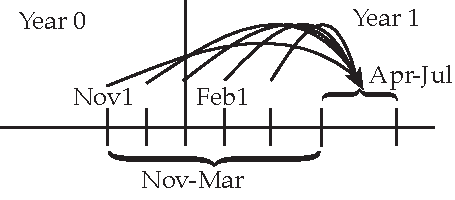
\includegraphics[width=.6\textwidth]{figs/one-year.pdf} 
		\end{block}
      \end{column}
        
      %%%%%%%%%%%%%%%%%%%%%%%%%%%%%%%%%%%%%%%%%%%%%%%%%%%%%%%%%%%%%%%%%%%%
      %
      % Column 2
      %
      %%%%%%%%%%%%%%%%%%%%%%%%%%%%%%%%%%%%%%%%%%%%%%%%%%%%%%%%%%%%%%%%%%%%
        \begin{column}{.33\linewidth}
        	%%%%%%%%%%%%%
        %%%%% Block 1
        %%%%%%%%%%%%%
        \begin{block}{\large The Interannual Forecasting Dilema}
        
			\begin{itemize}
				\item On the interannual time scale, {\color{orange}climate/snowpack information 
				      is poor} or not available
				\item A logical step is to use traditional time series methods, ARMA, KNN, MC 
				      but {\color{orange}Traditional methods provide little or no 
				      predictability over climatology} (trust me, I've tried)
				\item Snow, Climate {\color{orange}predictors and seasonal flow timeseries have 
				      very low autocorrelation} (Lees Ferry, show below, AC=0.26)
							
			\end{itemize}
			
			\begin{columns}
				\begin{column}{.48\textwidth}
					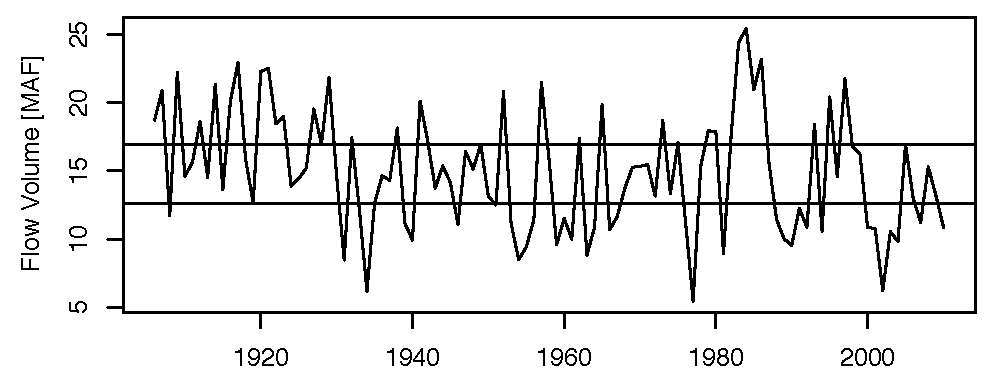
\includegraphics[width=\textwidth]{figs/lees.pdf} 
				
					\centerline{Annual Naturalized flow at Lees Ferry. }

				\end{column}
				\begin{column}{.49\textwidth}

					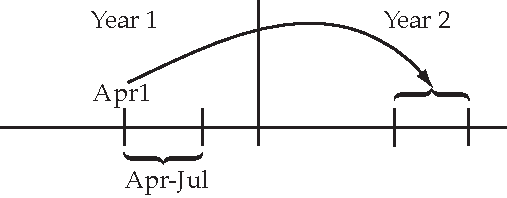
\includegraphics[width=.9\textwidth]{figs/two-year.pdf}
					
					Goal to make predictions from Apr 1 of the following year of Lees Ferry Flow.
				\end{column}
			\end{columns}
			 
		\end{block}
		
		%%%%%%%%%%%%%
        %%%%% Block 2
        %%%%%%%%%%%%%
		\begin{block}{Hidden Markov Models}
			\begin{columns}
				\begin{column}{.48\textwidth}
					$$\text{Pr}(C_t|\mathbf{C}^{(t-1)})=\text{Pr}(C_t|C_{t-1}), t=2,3,...$$
					$$\text{Pr}(X_t|\mathbf{X}^{(t-1)},\mathbf{C}^{(t)})=\text{Pr}(X_t|C_{t}), t\in	
					  \mathbb{N}$$
					  
					  \centering
					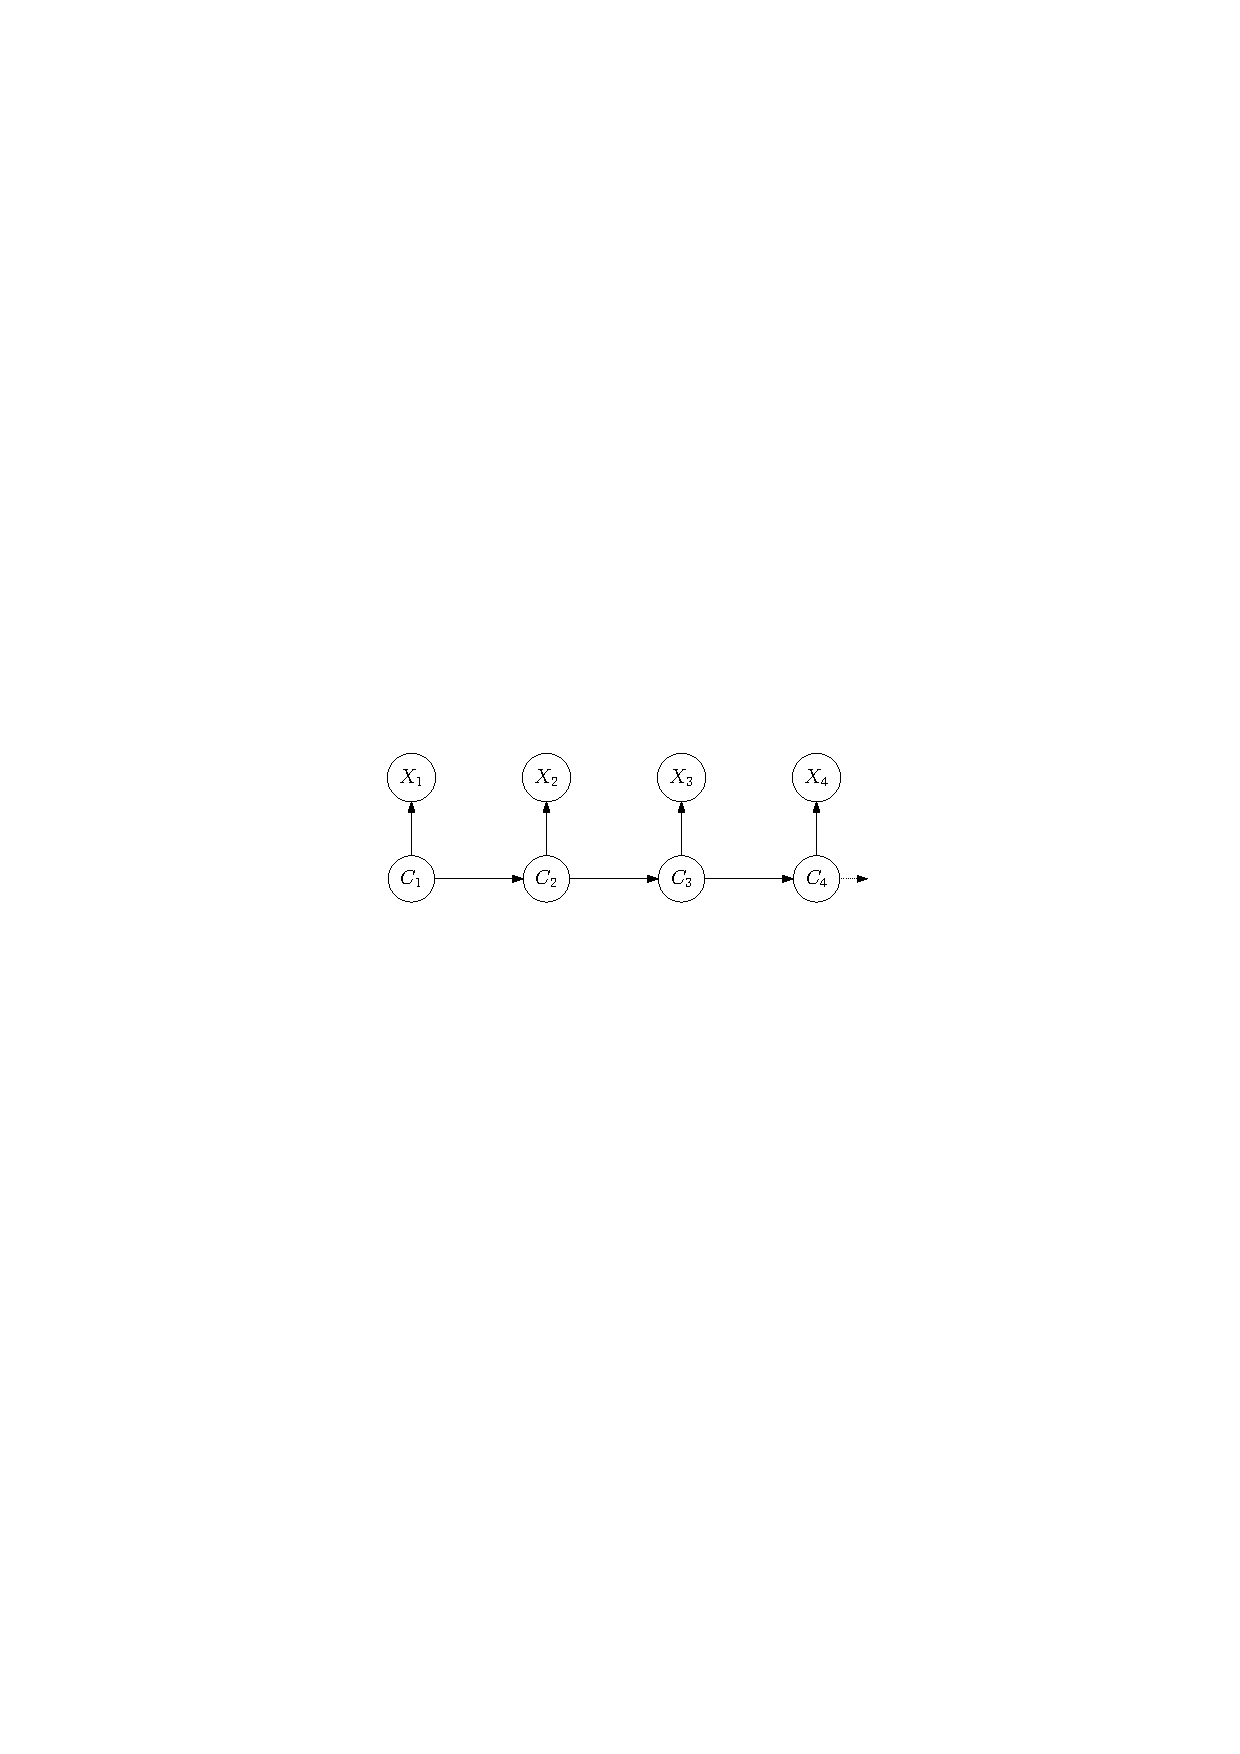
\includegraphics[width=\textwidth]{figs/hmm-digraph.pdf}

				\end{column}
				\begin{column}{.48\textwidth}
				\begin{itemize}
			    \item General time series model
				\item Markov process determines `hidden' state, state dictates component 
				      distribution
				\item A model that includes discrete states makes intuitive sense given the 
				      concept of climate regimes (such as El Ni$\tilde{\mbox{n}}$o) and has 
				      flexibility over explicit MC states.
			\end{itemize}
				\end{column}
			\end{columns}
			  			
		%\end{block}
		

		%\begin{block}{Hidden Markov Models}
			\begin{columns}
				\begin{column}{.58\textwidth}
					\centering
					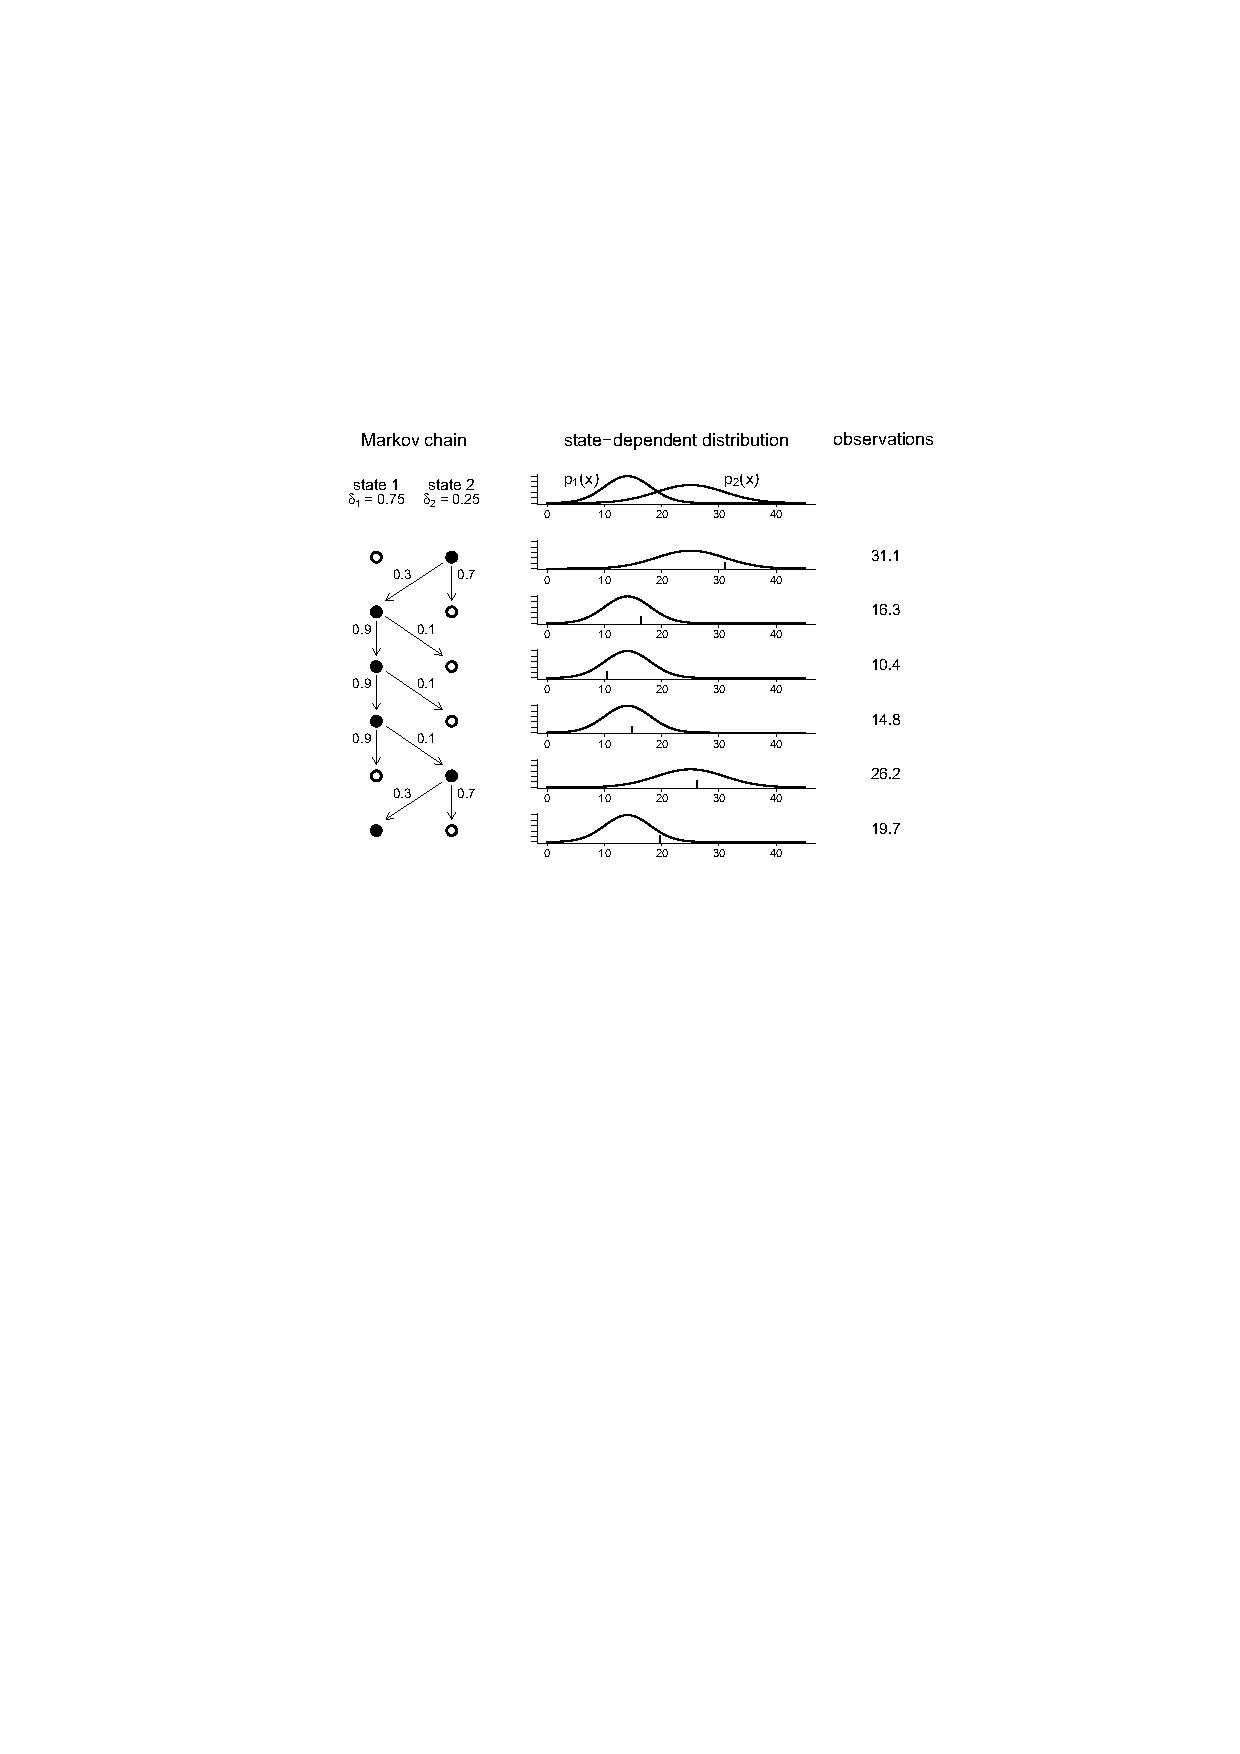
\includegraphics[width=.8\textwidth]{figs/hmm-diagram.pdf}
					
					(\small{Image from Zucchini and MacDonald, 2009}). 
				\end{column}
				\begin{column}{.38\textwidth}
					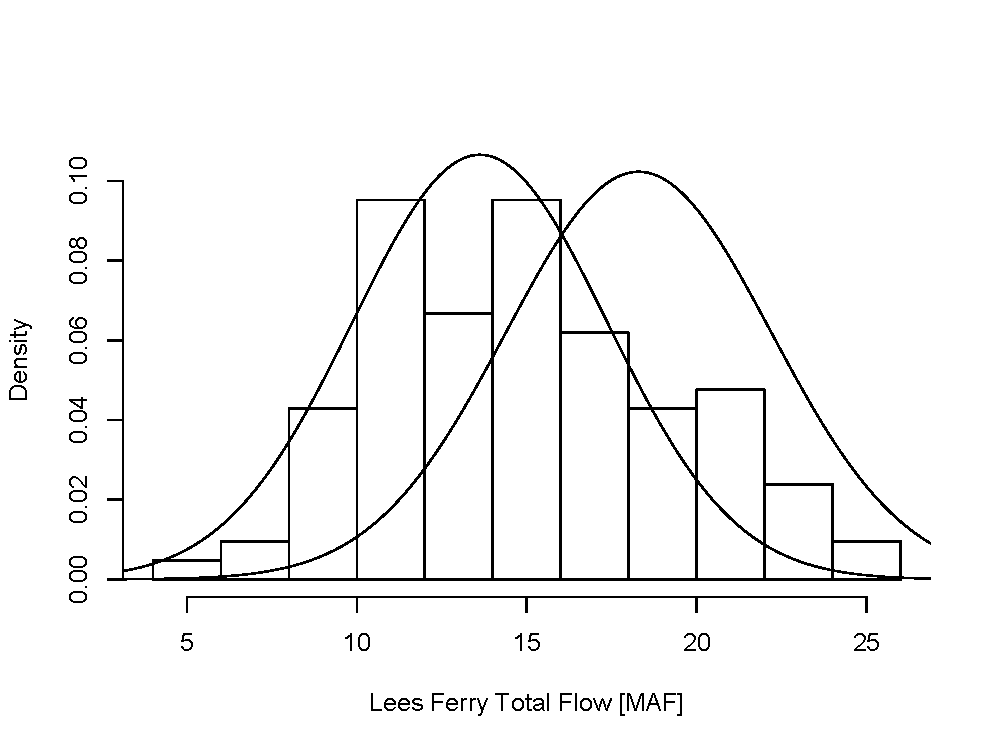
\includegraphics[width=\textwidth]{figs/hmm-2state-pdf.pdf}
					
					HMM(2) fit to Lees Ferry data. 
				\end{column}
			\end{columns}
		\end{block}
		
		%%%%%%%%%%%%%
        %%%%% Block 3
        %%%%%%%%%%%%%
		\begin{block}{HMM Forecasting Results}
			\begin{columns}
				\begin{column}{.58\textwidth}
				
					Forecasts made using {\color{orange}HMMs provide an overall 15\% improvement
					over climatology}. 
					\centerline{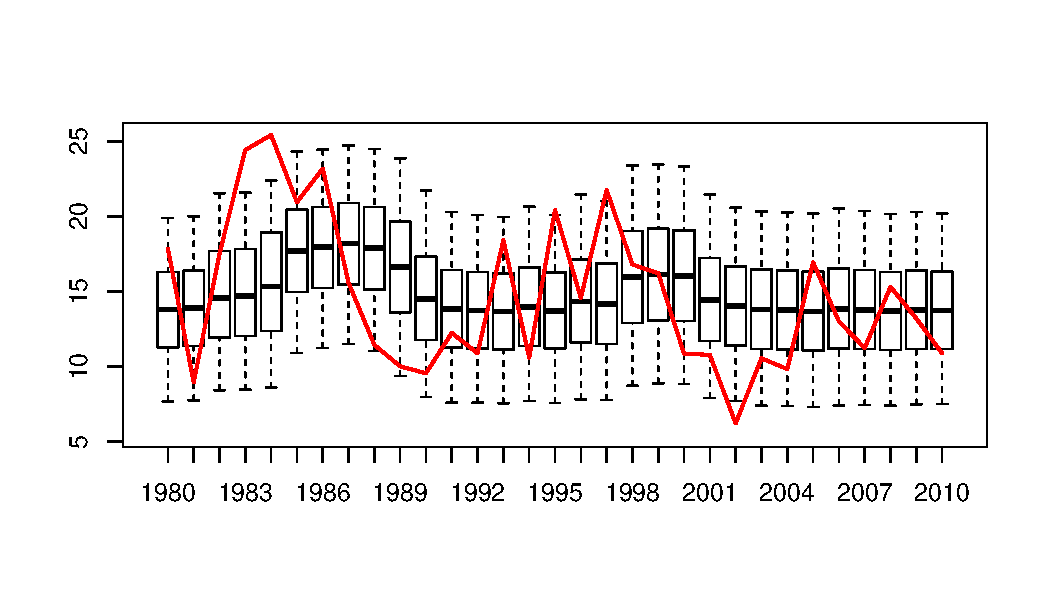
\includegraphics[width=\textwidth]{figs/hmm-order-2.pdf}}
					
					HMMs also show favorable shifts in exceedance probability.
				\end{column}
				\begin{column}{.38\textwidth}
					\centerline{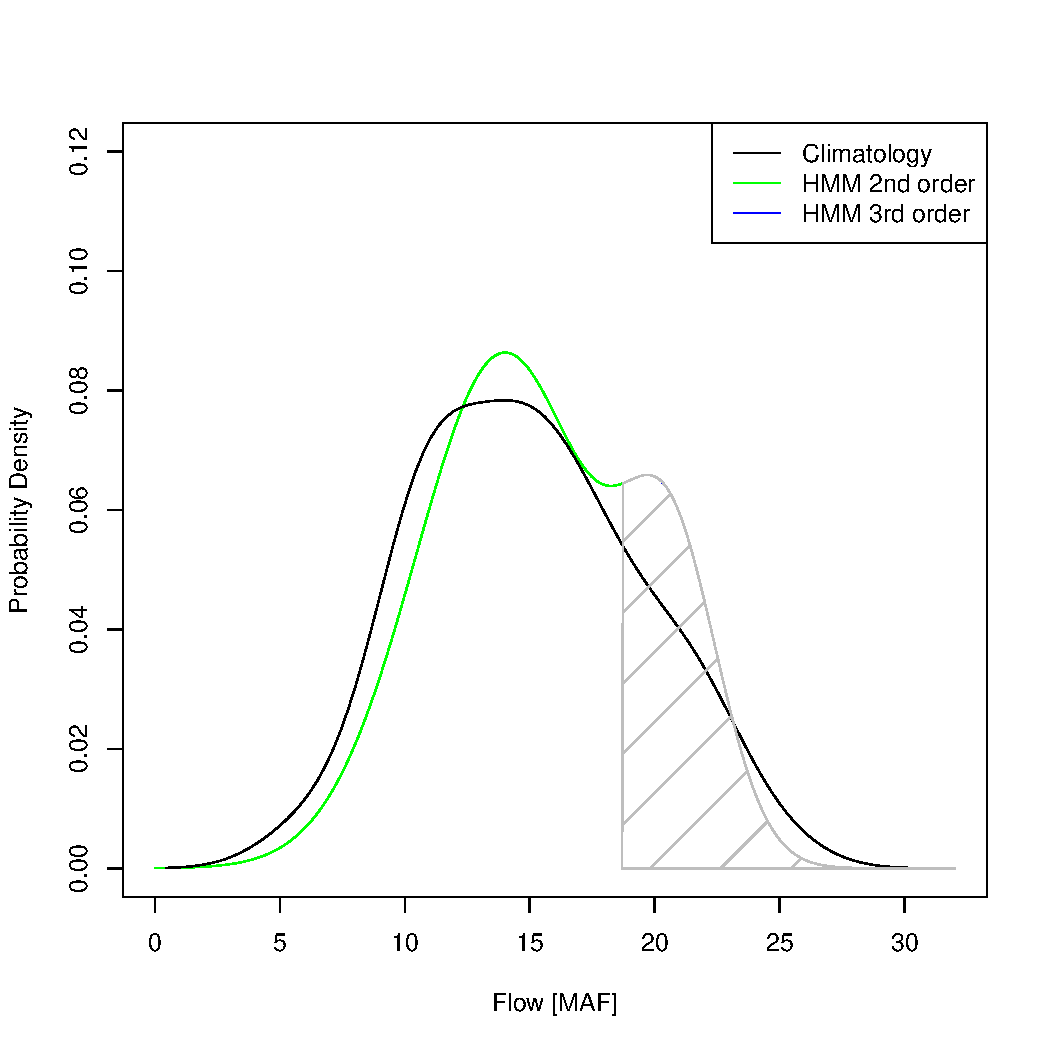
\includegraphics[width=\textwidth]{figs/pdf-shift1984.pdf}}
					
				  Eg. 1984 actual flow $\approx$23 MAF. Overall Climatology percent exceedance 
				  10\%;  HMM(2), 14\%
				\end{column}
			\end{columns}
		\end{block}
		
      \end{column}
      
      %%%%%%%%%%%%%%%%%%%%%%%%%%%%%%%%%%%%%%%%%%%%%%%%%%%%%%%%%%%%%%%%%%%%
      %
      % Column 3
      %
      %%%%%%%%%%%%%%%%%%%%%%%%%%%%%%%%%%%%%%%%%%%%%%%%%%%%%%%%%%%%%%%%%%%%
      \begin{column}{.33\linewidth}
      
	    %%%%%%%%%%%%%
        %%%%% Block 1
        %%%%%%%%%%%%%
		\begin{block}{Global Decoding Results}
		
			\begin{columns}
				\begin{column}{.38\textwidth}
					The most likely sequence of hidden states of the fitted HMM is called the Global Decoding. The global decoding of the Lees Ferry time series provides insight into the {\color{orange}long-term persistant ``regime-switching''} behavior of the system. 
				\end{column}
				\begin{column}{.58\textwidth}
					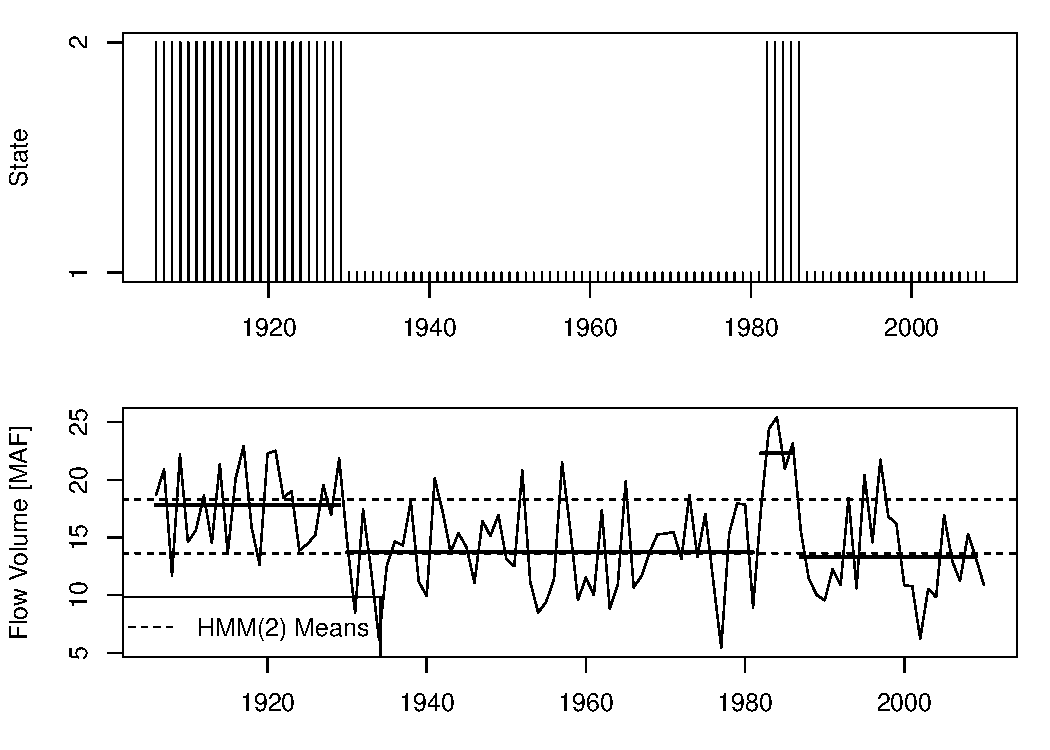
\includegraphics[width=\textwidth]{figs/decoding-period-means.pdf}
				\end{column}
			\end{columns}
			
		\end{block}
		
		%%%%%%%%%%%%%
        %%%%% Block 2
        %%%%%%%%%%%%%
		\begin{block}{Simulation with Hidden Markov Models}
		\begin{columns}
			\begin{column}{.48\textwidth}
				\begin{itemize}
					\item HMMs are also useful for simulation (used in risk analysis). 
					\item Alternative to AR simulations or ISM
					\item Can we capture longer period variability?
				\end{itemize}
			\end{column}
			\begin{column}{.48\textwidth}
				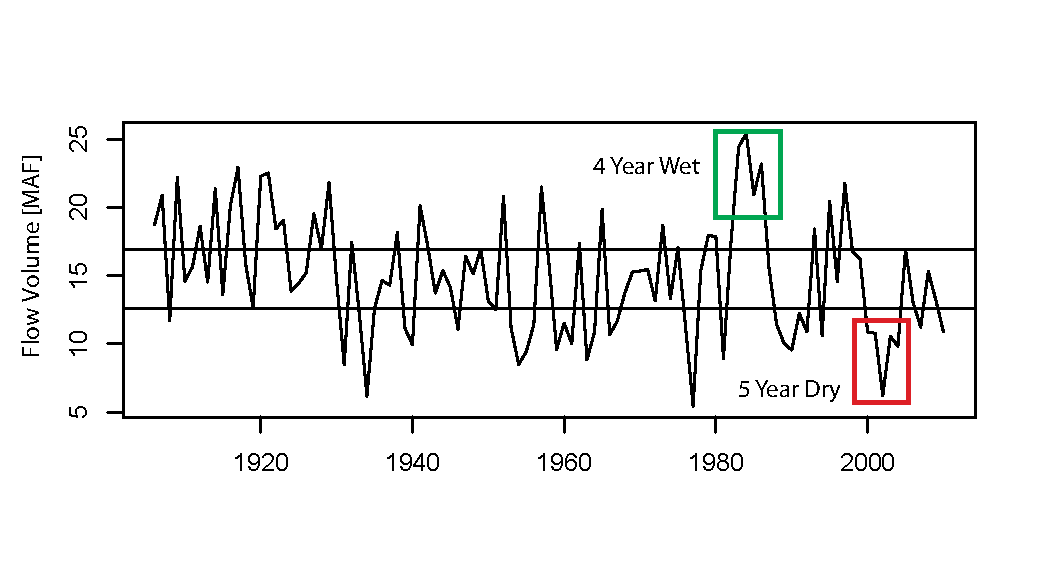
\includegraphics[width=\textwidth]{figs/lees-5yrdry.pdf}
			\end{column}
		\end{columns}
		
		\begin{columns}
			\begin{column}{.48\textwidth}
				\centerline{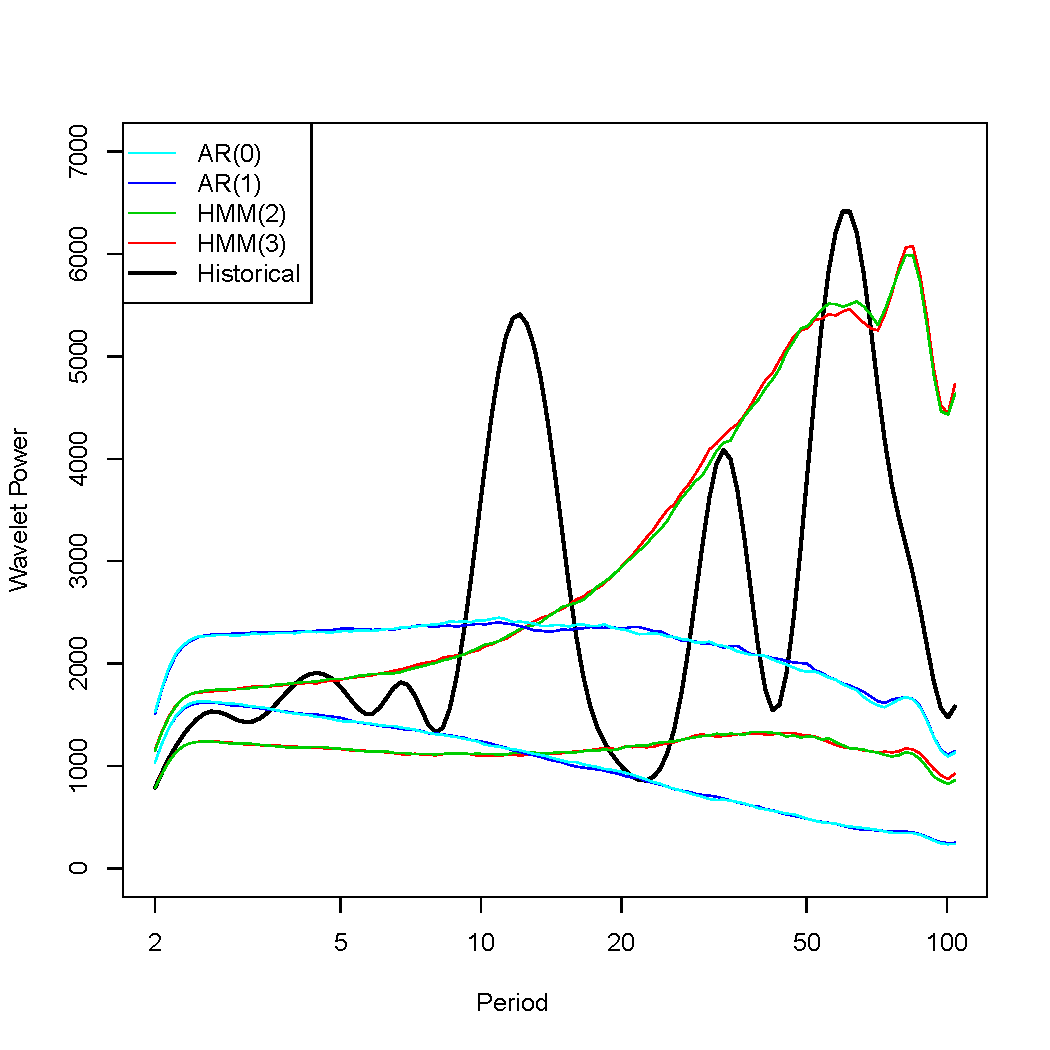
\includegraphics[width=\textwidth]{figs/spectrum.pdf}}

			\end{column}
			\begin{column}{.48\textwidth}
				\centerline{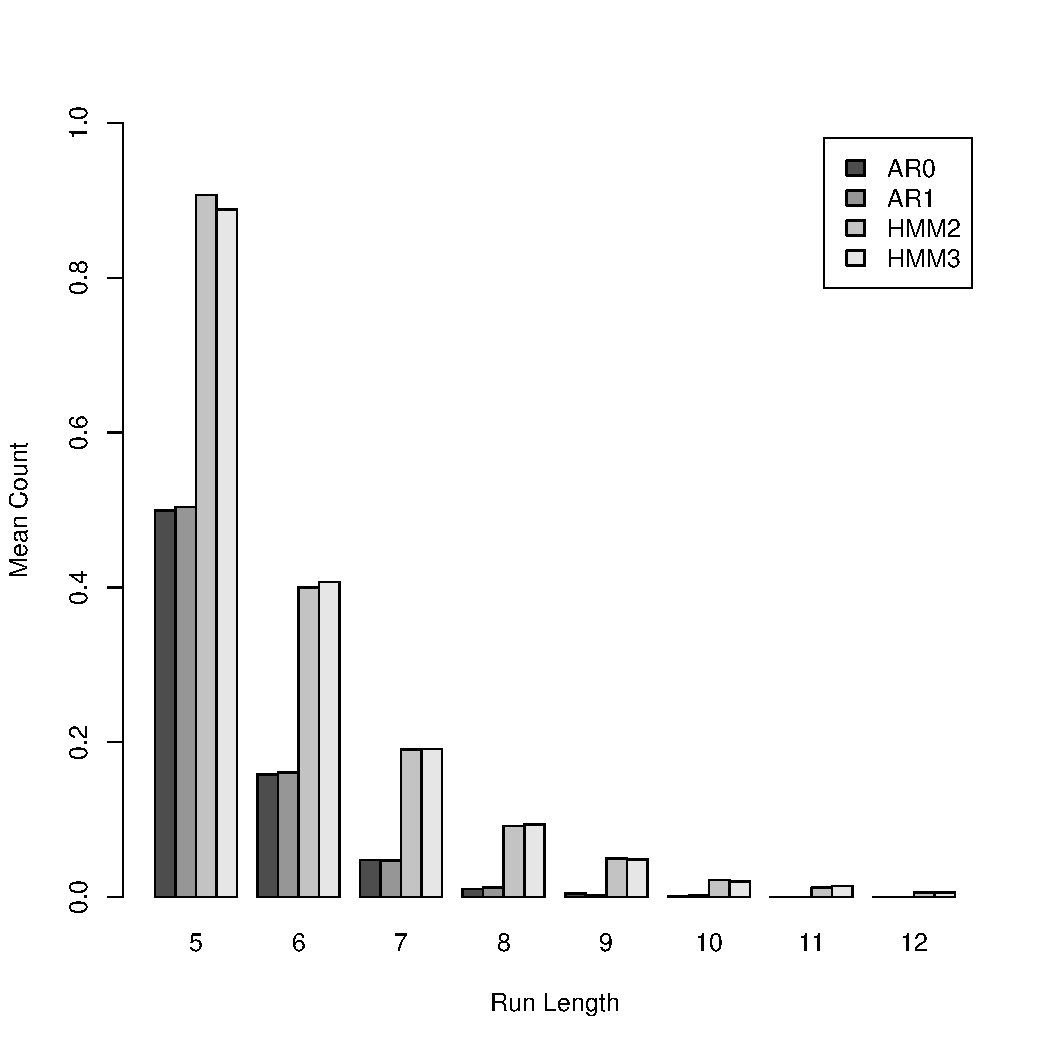
\includegraphics[width=\textwidth]{figs/sim-lengths-mean.pdf}}
			\end{column}
		\end{columns}
		Ability to capture longer period variability as well as observed statistics (not shown).
		\end{block}
		
		%%%%%%%%%%%%%
        %%%%% Block 3
        %%%%%%%%%%%%%
        \begin{block}{Conclusions}
        	
			\begin{itemize}
				\item Interannual forecasting in the Upper Colorado River Basin with Hidden 
				    Markov models shows forecast improvements over traditional time series 
				    models. 	
				\item HMMs capture long term underlying persistance in the system as well as 
					observed statistics.
			\end{itemize}
        
        \end{block}
        
        %%%%%%%%%%%%%
        %%%%% Block 3
        %%%%%%%%%%%%%
        %\begin{block}{Future Work}
        	%
		%	\begin{itemize}
		%		\item Disaggregation.
		%		\item Run through dicision model. 
		%	\end{itemize}
        %
        %\end{block}
        
        %%%%%%%%%%%%%
        %%%%% Block 4
        %%%%%%%%%%%%%
        \begin{block}{References}
        	\small
		\begin{itemize}
	        \item Bracken, C., B. Rajagopalan, and J. Prairie (2010), A multisite seasonal ensemble streamflow fore¬casting technique, Water Resour. Res, 46(3), W03,532, doi:10.1029/2009WR007965. 
	        
	        \item Regonda, S. K., B. Rajagopalan, M. Clark, and E. Zagona (2006), A multimodel ensemble forecast framework: Application to spring seasonal flows in the Gunnison river basin, Water Resour. Res, 
	42. 
	        \item Zucchini, W. (2009). Hidden Markov models for time series: an introduction using R.
        \end{itemize}
        \end{block}
        \vspace{1.1cm}

      
      \end{column}
    \end{columns}
  \end{frame}
\end{document}


